\documentclass{beamer}

\usepackage{tikz}
\usetikzlibrary{patterns}
\usetikzlibrary{calc}
\usetikzlibrary{shapes, arrows, positioning}

\usepackage{tabularray}
\UseTblrLibrary{booktabs}
\DefTblrTemplate{contfoot-text}{normal}{\lang{(Continued on next page)}{(Continua na próxima página)}} 
\SetTblrTemplate{contfoot-text}{normal} 
\DefTblrTemplate{conthead-text}{normal}{\lang{(continued)}{(continuação)}} 
\SetTblrTemplate{conthead-text}{normal}

\usepackage{enumitem}
\definecolor{ifscgreen}{RGB}{50,93,61}

\setlist[enumerate,1]{label=\colorbox{ifscgreen}{\textcolor{white}{\arabic*}}\quad, leftmargin=*}
\setlist[enumerate,2]{label=\colorbox{ifscgreen!70}{\textcolor{white}{\arabic{enumi}.\arabic*}}\quad, leftmargin=*}
\setlist[enumerate,3]{label=\colorbox{ifscgreen!40}{\textcolor{white}{\arabic{enumi}.\arabic{enumii}.\arabic*}}\quad, leftmargin=*}
% ------------------------------
% Codificação e idioma
% ------------------------------
% \usepackage[utf8]{inputenc}
\usepackage[T1]{fontenc}
\usepackage[brazil]{babel}

% ------------------------------
% Matemática e símbolos
% ------------------------------
\usepackage{amsmath}

% ------------------------------
% Gráficos e figuras
% ------------------------------
\usepackage{graphicx}
\usepackage{subfigure}

% ------------------------------
% Cores, URL e hiperlinks
% ------------------------------
\usepackage{url,color}
\usepackage{hyperref}
\hypersetup{
  pdfstartview={Fit},
  pdftitle={\@title},
  pdfsubject={Engenharia de Telecomunicacoes - IFSC},
  pdfauthor={\@author}
}

% ------------------------------
% Listagens e pseudocódigo
% ------------------------------
\usepackage[
plainruled,
noline
]{algorithm2e}

% ------------------------------
% Bibliografia
% ------------------------------
\usepackage[backend=biber,style=numeric,citestyle=ieee]{biblatex}
\addbibresource{references.bib}
\setbeamertemplate{bibliography item}{\insertbiblabel}

% ------------------------------
% Outros pacotes
% ------------------------------
\usepackage{ifsc} % (pacote personalizado, ok manter)

% ------------------------------
% Macros e comandos personalizados
% ------------------------------
\newcommand{\tab}[1]{\hspace{.2\textwidth}\rlap{#1}}

\newcommand{\DAY}{\the\day}
\newcommand{\MONTH}{%
  \ifcase\the\month
  \or Janeiro%
  \or Fevereiro%
  \or Março%
  \or Abril%
  \or Maio%
  \or Junho%
  \or Julho%
  \or Agosto%
  \or Setembro%
  \or Outubro%
  \or Novembro%
  \or Dezembro%
  \fi}
\newcommand{\YEAR}{\the\year}

% ------------------------------
% Dados do título
% ------------------------------
\title{PRG203402 - Lógica de Programação:}
\subtitle{\LARGE Introdução ao Python}
\author{João Cláudio Elsen Barcellos}
\date{\scriptsize \DAY~de \MONTH~de \YEAR}
\institute{
  Engenheiro Eletricista\\
  Formado na Universidade Federal de Santa Catarina\\
  campus Florianópolis\\
  \url{joaoclaudiobarcellos@gmail.com}
}

% ------------------------------
% Customização das seções no Beamer
% ------------------------------
\def\sectionname{}
\def\insertsectionnumber{}
\def\subsectionname{}
\def\insertsubsectionnumber{}

\AtBeginSection[]{
  \begin{frame}
      \vfill
      \centering
      \begin{beamercolorbox}[sep=8pt,center,shadow=true,rounded=true]{title}
          \usebeamerfont{title}\insertsectionhead\par%
      \end{beamercolorbox}
      \vfill
  \end{frame}
}

\setbeamertemplate{caption}[numbered]

% ------------------------------
% Controle de idioma
% ------------------------------
\usepackage{ifthen}
\newboolean{english}
\setboolean{english}{false} % true = inglês, false = português

% Configuração de idioma e títulos
\ifthenelse{\boolean{english}}{
  \usepackage[english]{babel}
  \renewcommand{\figurename}{Figure}
  \renewcommand{\tablename}{Table}
  \SetAlgorithmName{Algorithm}{}{}
  
  \SetKwInput{KwData}{Input}
  \SetKwInput{KwResult}{Output}
  \SetKwIF{If}{ElseIf}{Else}{if}{then}{else if}{else}{end if}
  \SetKwFor{While}{while}{do}{end while}
  \SetKwFor{For}{for}{do}{end for}
  \SetKw{Return}{return}
}{
  \usepackage[brazil]{babel}
  \renewcommand{\figurename}{Figura}
  \renewcommand{\tablename}{Tabela}
  \SetAlgorithmName{Algoritmo}{}{}
  
  \SetKwInput{KwData}{Entrada}
  \SetKwInput{KwResult}{Saída}
  \SetKwIF{If}{ElseIf}{Else}{se}{então}{senão se}{senão}{fim}
  \SetKwFor{While}{enquanto}{faça}{fim}
  \SetKwFor{For}{para}{faça}{fim}
  \SetKw{Return}{retorna}
}
% Comando para alternar entre idiomas (inglês/português)
\newcommand{\lang}[2]{\ifbool{english}{#1}{#2}}
    
% Default fixed font does not support bold face
\DeclareFixedFont{\ttb}{T1}{txtt}{bx}{n}{8} % for bold
\DeclareFixedFont{\ttm}{T1}{txtt}{m}{n}{8}  % for normal

% Custom colors
\usepackage{color}
\definecolor{deepblue}{rgb}{0,0,0.5}
\definecolor{deepred}{rgb}{0.6,0,0}
\definecolor{deepgreen}{rgb}{0,0.5,0}

\usepackage{listings}

% Python style for highlighting
\newcommand\pythonstyle{\lstset{
language=Python,
basicstyle=\ttm,
morekeywords={self},              % Add keywords here
keywordstyle=\ttb\color{deepblue},
emph={MyClass,__init__},          % Custom highlighting
emphstyle=\ttb\color{deepred},    % Custom highlighting style
stringstyle=\color{deepgreen},
frame=tb,                         % Any extra options here
showstringspaces=false,
numbers=none 
}}


% Python environment
\lstnewenvironment{python}[1][]
{
\pythonstyle
\lstset{#1}
}
{}

% Python for external files
\newcommand\pythonexternal[2][]{{
\pythonstyle
\lstinputlisting[#1]{#2}}}

% Python for inline
\newcommand\pythoninline[1]{{\pythonstyle\lstinline!#1!}}    
    
    \lstset{
      inputencoding = utf8,  % Input encoding
      extendedchars = true,  % Extended ASCII
      literate      =        % Support additional characters
      {á}{{\'a}}1  {é}{{\'e}}1  {í}{{\'i}}1 {ó}{{\'o}}1  {ú}{{\'u}}1
      {Á}{{\'A}}1  {É}{{\'E}}1  {Í}{{\'I}}1 {Ó}{{\'O}}1  {Ú}{{\'U}}1
      {à}{{\`a}}1  {è}{{\`e}}1  {ì}{{\`i}}1 {ò}{{\`o}}1  {ù}{{\`u}}1
      {À}{{\`A}}1  {È}{{\`E}}1  {Ì}{{\`I}}1 {Ò}{{\`O}}1  {Ù}{{\`U}}1
      {ä}{{\"a}}1  {ë}{{\"e}}1  {ï}{{\"i}}1 {ö}{{\"o}}1  {ü}{{\"u}}1
      {Ä}{{\"A}}1  {Ë}{{\"E}}1  {Ï}{{\"I}}1 {Ö}{{\"O}}1  {Ü}{{\"U}}1
      {â}{{\^a}}1  {ê}{{\^e}}1  {î}{{\^i}}1 {ô}{{\^o}}1  {û}{{\^u}}1
      {Â}{{\^A}}1  {Ê}{{\^E}}1  {Î}{{\^I}}1 {Ô}{{\^O}}1  {Û}{{\^U}}1
      {œ}{{\oe}}1  {Œ}{{\OE}}1  {æ}{{\ae}}1 {Æ}{{\AE}}1  {ß}{{\ss}}1
      {ẞ}{{\SS}}1  {ç}{{\c{c}}}1 {Ç}{{\c{C}}}1 {ø}{{\o}}1  {Ø}{{\O}}1
      {å}{{\aa}}1  {Å}{{\AA}}1  {ã}{{\~a}}1  {õ}{{\~o}}1 {Ã}{{\~A}}1
      {Õ}{{\~O}}1  {ñ}{{\~n}}1  {Ñ}{{\~N}}1  {¿}{{?`}}1  {¡}{{!`}}1
      {„}{\quotedblbase}1 {“}{\textquotedblleft}1 {–}{$-$}1
      {°}{{\textdegree}}1 {º}{{\textordmasculine}}1 {ª}{{\textordfeminine}}1
      {£}{{\pounds}}1  {©}{{\copyright}}1  {®}{{\textregistered}}1
      {«}{{\guillemotleft}}1  {»}{{\guillemotright}}1  {Ð}{{\DH}}1  {ð}{{\dh}}1
      {Ý}{{\'Y}}1    {ý}{{\'y}}1    {Þ}{{\TH}}1    {þ}{{\th}}1    {Ă}{{\u{A}}}1
      {ă}{{\u{a}}}1  {Ą}{{\k{A}}}1  {ą}{{\k{a}}}1  {Ć}{{\'C}}1    {ć}{{\'c}}1
      {Č}{{\v{C}}}1  {č}{{\v{c}}}1  {Ď}{{\v{D}}}1  {ď}{{\v{d}}}1  {Đ}{{\DJ}}1
      {đ}{{\dj}}1    {Ė}{{\.{E}}}1  {ė}{{\.{e}}}1  {Ę}{{\k{E}}}1  {ę}{{\k{e}}}1
      {Ě}{{\v{E}}}1  {ě}{{\v{e}}}1  {Ğ}{{\u{G}}}1  {ğ}{{\u{g}}}1  {Ĩ}{{\~I}}1
      {ĩ}{{\~\i}}1   {Į}{{\k{I}}}1  {į}{{\k{i}}}1  {İ}{{\.{I}}}1  {ı}{{\i}}1
      {Ĺ}{{\'L}}1    {ĺ}{{\'l}}1    {Ľ}{{\v{L}}}1  {ľ}{{\v{l}}}1  {Ł}{{\L{}}}1
      {ł}{{\l{}}}1   {Ń}{{\'N}}1    {ń}{{\'n}}1    {Ň}{{\v{N}}}1  {ň}{{\v{n}}}1
      {Ő}{{\H{O}}}1  {ő}{{\H{o}}}1  {Ŕ}{{\'{R}}}1  {ŕ}{{\'{r}}}1  {Ř}{{\v{R}}}1
      {ř}{{\v{r}}}1  {Ś}{{\'S}}1    {ś}{{\'s}}1    {Ş}{{\c{S}}}1  {ş}{{\c{s}}}1
      {Š}{{\v{S}}}1  {š}{{\v{s}}}1  {Ť}{{\v{T}}}1  {ť}{{\v{t}}}1  {Ũ}{{\~U}}1
      {ũ}{{\~u}}1    {Ū}{{\={U}}}1  {ū}{{\={u}}}1  {Ů}{{\r{U}}}1  {ů}{{\r{u}}}1
      {Ű}{{\H{U}}}1  {ű}{{\H{u}}}1  {Ų}{{\k{U}}}1  {ų}{{\k{u}}}1  {Ź}{{\'Z}}1
      {ź}{{\'z}}1    {Ż}{{\.Z}}1    {ż}{{\.z}}1    {Ž}{{\v{Z}}}1  {ž}{{\v{z}}}1
      % ¿ and ¡ are not correctly displayed if inconsolata font is used
      % together with the lstlisting environment. Consider typing code in
      % external files and using \lstinputlisting to display them instead.      
    }
    
\begin{document}

\captionsetup{labelformat=empty}

\begin{frame}[t]
    % Example of a note:
    % \note{Boa tarde a todos, na aula de hoje iremos estudar os circuitos sequenciais...}
    \maketitle
    \vspace{-1cm}
    \begin{flushleft}
        \vfill
        \textit{\tiny $^{*}$Créditos ao Prof. Emerson Ribeiro de Mello, o qual criou e disponibilizou o template aqui usado, via ShareLaTeX}\par
        \textit{\tiny $^{**}$Créditos ao Prof. Renan Augusto Starke, o qual forneceu parte do conteúdo usado nesta apresentação}
    \end{flushleft}
\end{frame}

\begin{frame}[t]{Na aula de hoje veremos...}
    \tableofcontents
\end{frame}

\begin{frame}

\begin{center}

\includegraphics[scale=0.3]{./figures/python-logo.png}
\end{center}
  
  \begin{itemize}
   \vfill \item Python é uma das \textbf{cinco} mais populares linguagens de programação (segundo índice \href{http://www.tiobe.com/tiobe-index/}{TIOBE}). 
   \vfill \item É mais fácil de entender do que Java ou C.
   \vfill \item Menos trabalho para fazer gráficos.
   \vfill \item Tudo que se aprende em Python é aplicado a outras linguagens.
  \end{itemize} 

\end{frame}


\begin{frame}

\begin{center}

\includegraphics[scale=0.3]{./figures/python-logo.png}
\end{center}
  
  \begin{itemize}
   \vfill \item Há duas versões principais de Python: 2 e 3.
   
   \vfill \item Há diferenças entre as duas, utilizaremos a versão 3.
   
   \vfill \item Sempre verifique a versão utilizada.
   
  \end{itemize}
\end{frame}

\begin{frame}{Python: por onde começar}
 
 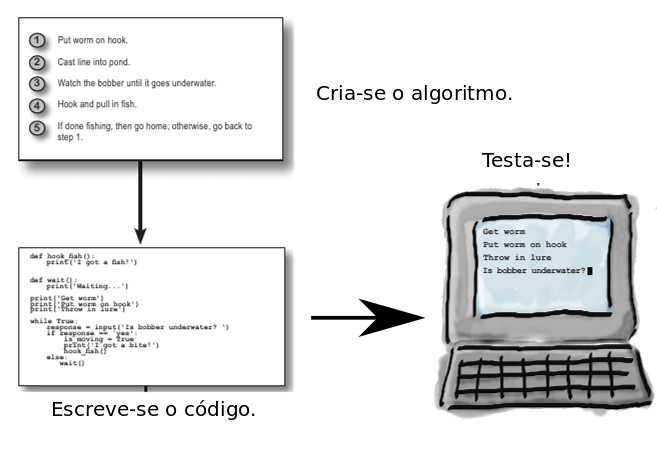
\includegraphics[scale=0.4]{./figures/fluxo.png}
 
\end{frame}

\begin{frame}{Python: por onde começar}
 
 \begin{itemize}
  \vfill \item No MacOS e Linux já está instalado nativamente.
  \vfill \item Windows, sugere-se instalar o \href{https://www.anaconda.com/distribution/}{Anaconda}.
  \vfill \item Um programa em Python é um arquivo de texto simples, pode-se escrever em qualquer programa.
  
  \begin{itemize}
   \vfill\item Mas há editores especiais que ajudam na codificação.
   \vfill\item Inclusive online: \href{https://pynative.com/online-python-code-editor-to-execute-python-code/}{Python Online}
  \end{itemize}  
 \end{itemize}
\end{frame}


\begin{frame}{Idle3}
 \begin{center}
  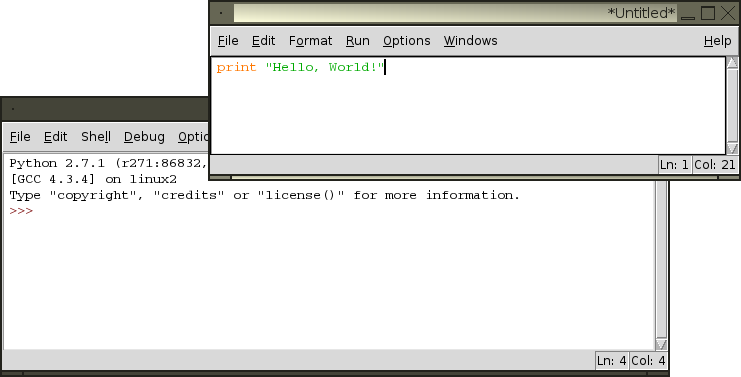
\includegraphics[scale=0.8]{./figures/idle3.png}
 \end{center}
\end{frame}

\begin{frame}{PyCharm}
 \begin{center}
  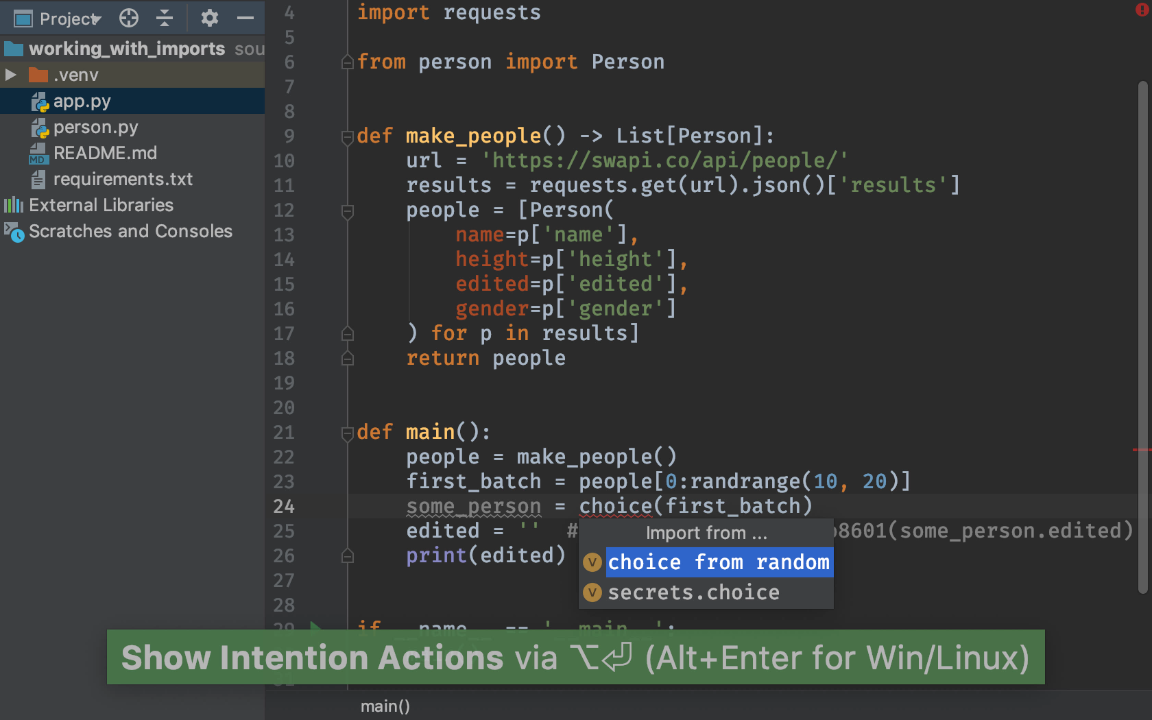
\includegraphics[scale=0.4]{./figures/pycharm.png}
 \end{center}
\end{frame}

\begin{frame}{Spyder}
 \begin{center}
  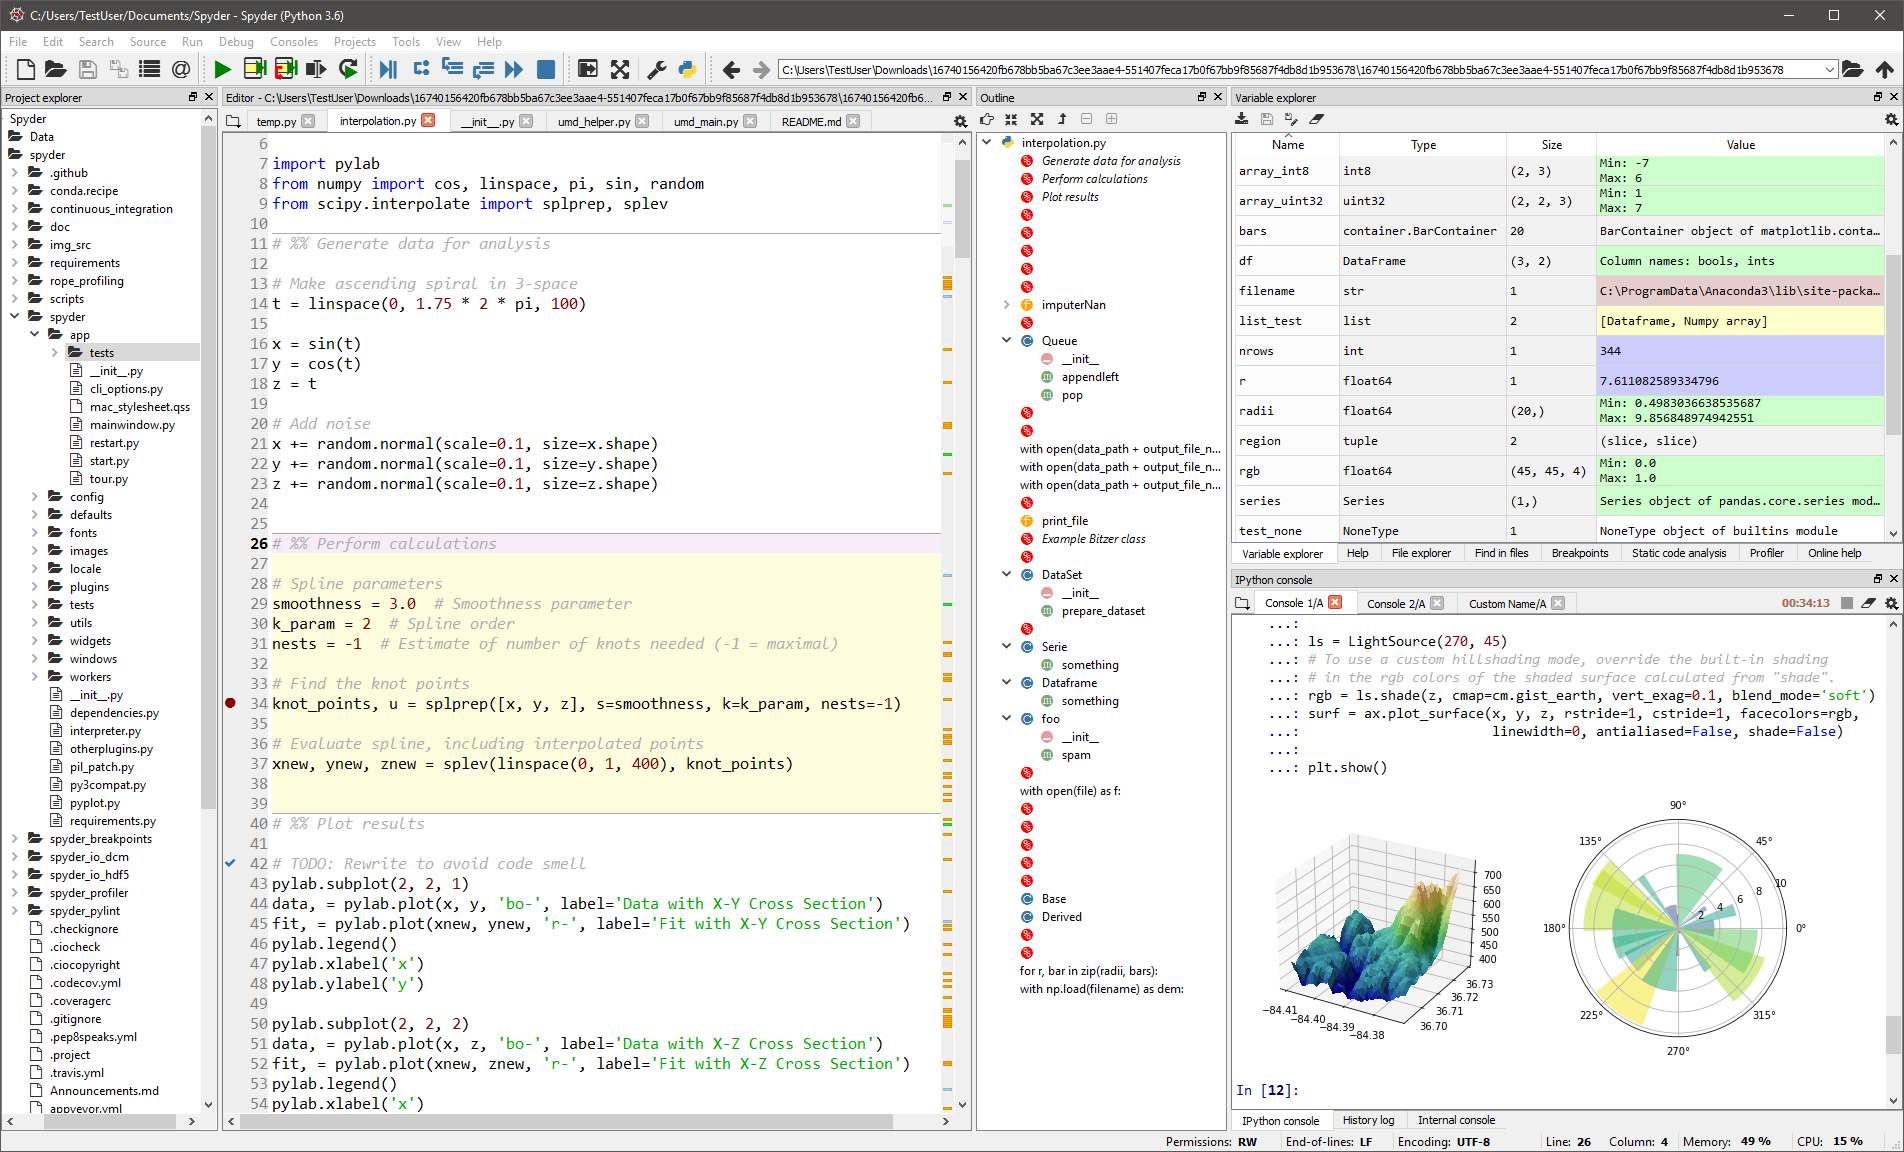
\includegraphics[scale=0.2]{./figures/spyder.png}
 \end{center}
\end{frame}

\begin{frame}{Visual Code}
 \begin{center}
  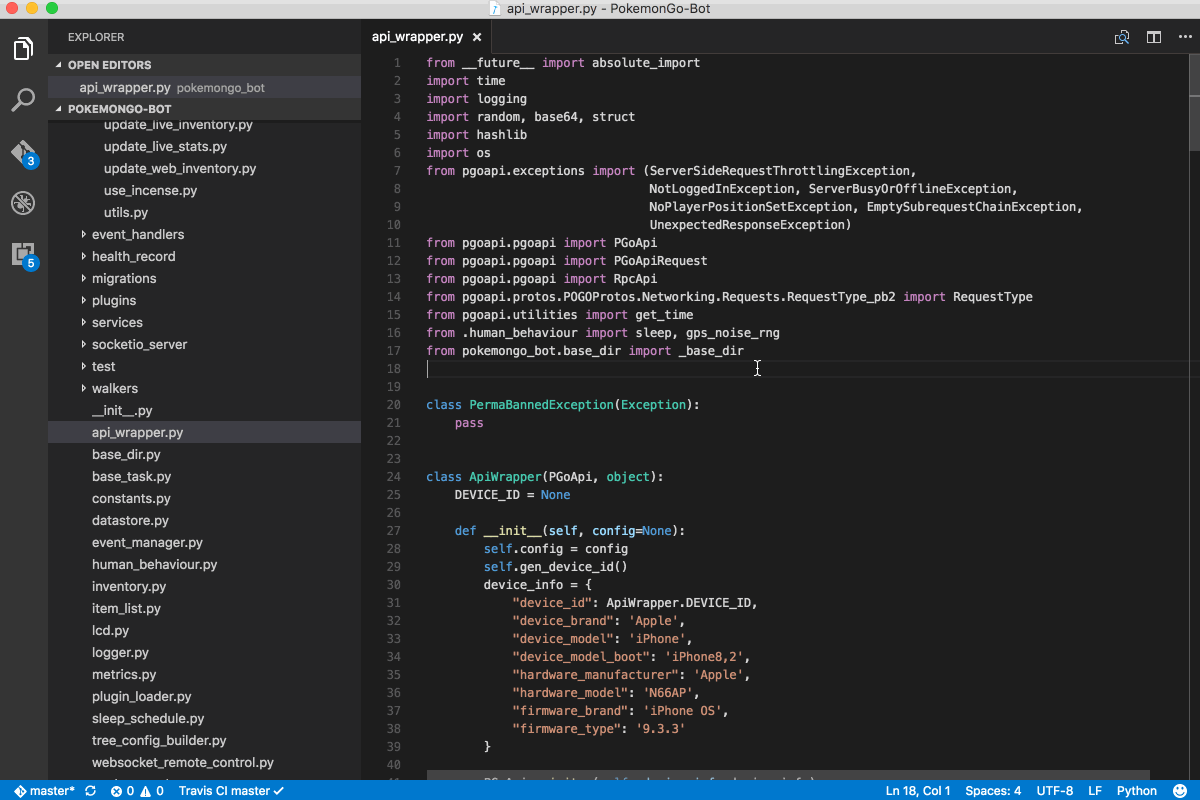
\includegraphics[scale=0.4]{./figures/vscode.png}
 \end{center}
\end{frame}

\begin{frame}{Jupyter Notebook}
 \begin{center}
  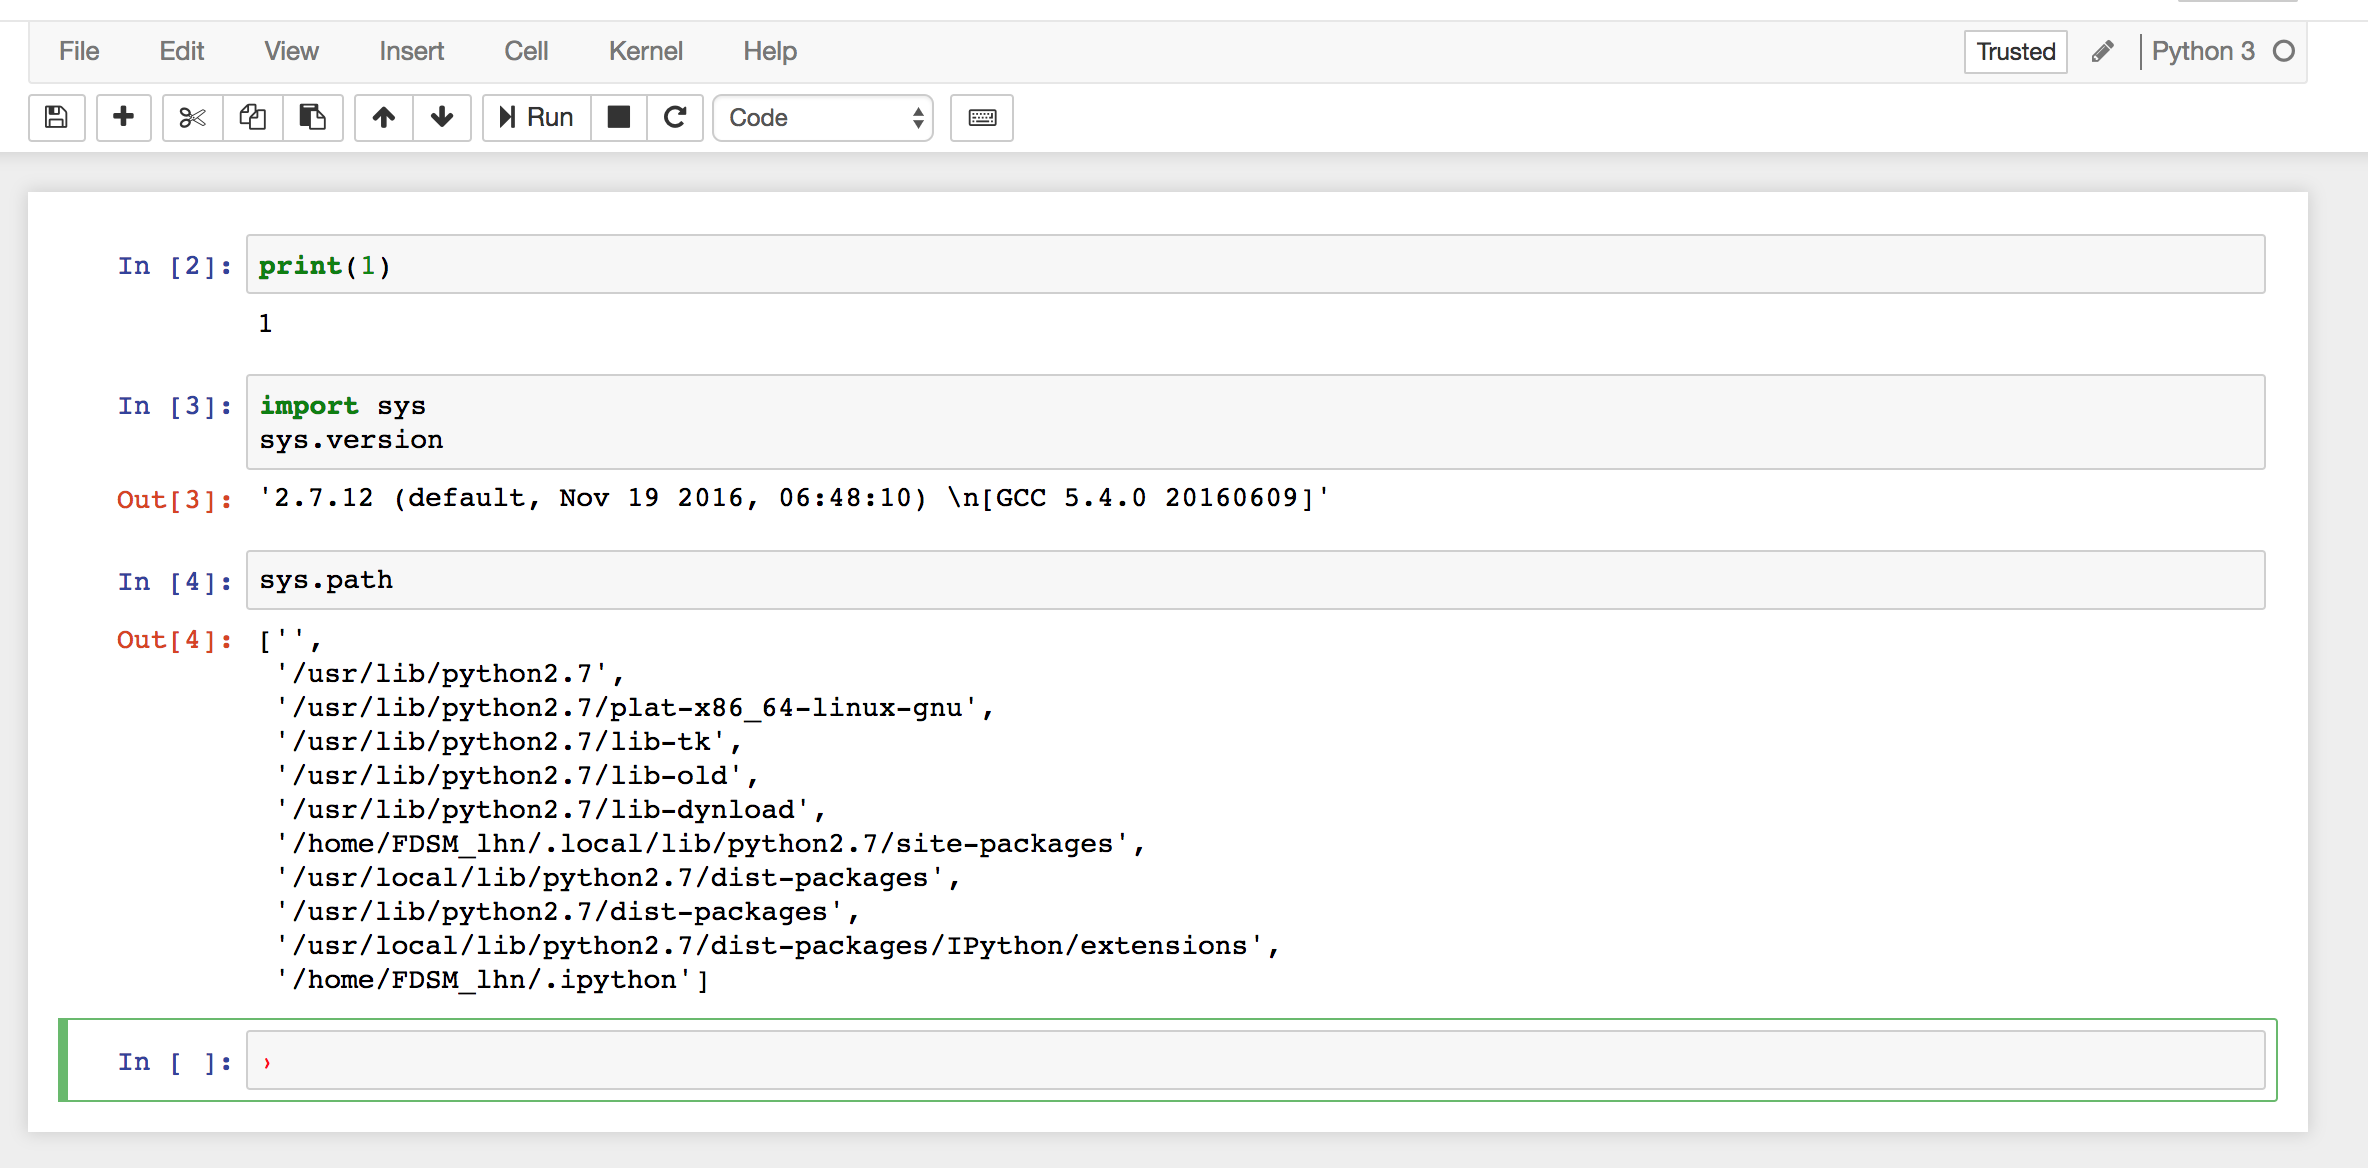
\includegraphics[scale=0.4]{./figures/jupyter.png}
 \end{center}
\end{frame}


\begin{frame}[fragile]
  \frametitle{Meu primeiro programa}  
  \begin{itemize}
    \vfill \item Tradicionalmente o primeiro programa escrito é um \textcolor{red}{``Olá Mundo''}.
    \vfill \item Para introduzir você ao mundo em Python:
  \end{itemize}

\vfill \begin{python}
print("Olá mundo, meu nome é Juquinha")
\end{python}

\end{frame}

\begin{frame}[fragile]
  \frametitle{Comentários}

  \begin{itemize}
    \vfill \item Comentários são ignorados pelo computador quando um programa é executado.
    \vfill \item Eles ajudam na compreensão do código.
    \vfill \item Comentários em Python são ativados pelo caractere: \textcolor{red}{\#}
  \end{itemize}

\vfill \begin{python}
# Isso é um comentário
print("Olá!")  # A partir daqui também é!

print("# isso não é comentário")
# Um novo comentário pode ser colocado aqui!
\end{python}

\end{frame}


\begin{frame}[fragile]
  \frametitle{A função print}

  \begin{itemize}
    \vfill \item A função \textcolor{blue}{print} imprime dados do programa.
    \vfill \item Funções em Python são parecidas com as matemáticas:
    \begin{itemize}
      \item seno(x)
      \item cosseno(x)
      \item f(x)
    \end{itemize}
    \vfill \item Funções são sempre seguidas por parênteses \textcolor{red}{(   )}
    \vfill \item Os dados colocados entre parênteses são conhecidos como \textbf{argumentos}. 
    
  \end{itemize}
\end{frame}

\begin{frame}[fragile]
  \frametitle{Personalizando o print}

  \begin{itemize}
    \item Há alguns caracteres especiais:
  \end{itemize}

\vfill \begin{python}
# Se eu precisar imprimir o caractere " 
# Devo colocar uma barra na frente
print("Desejo imprimir o \" por algum motivo.")

# E se eu quiser o caractere \ ?
print("Esse arquivo está em C:\\minha_pasta")
\end{python}
\end{frame}

\begin{frame}[fragile]
  \frametitle{Personalizando o print}

  \begin{center}
  \begin{tabular}{l|l}
    Caractere & Descrição \\ \hline
    \textbackslash ' & Aspas simples \\
    \textbackslash " & Aspas duplas \\
    \textbackslash t & Tabulação \\
    \textbackslash n & Nova linha \\
  \end{tabular}
  \end{center}

\vfill \begin{python}
 print("Isso\né\num\nexemplo.")
\end{python}

\vfill \begin{python}
  Isto
  é
  um
  exemplo.
\end{python}  
\end{frame}

\begin{frame}[fragile]
  \frametitle{Variáveis}

  \begin{itemize}
    \vfill \item Uma \textbf{variável} é utilizada para guardar dados que serão reutilizados. 
    \vfill \item Para criar uma variável em Python, utilizamos o operador de atribuição \textcolor{red}{=} 
  \end{itemize}

\vfill \begin{python}
x = 5
print(x)  # Isto irá imprimir 5

mensagem = "Olá"
print(mensagem) # Isto irá imprimir Olá
\end{python}  
\end{frame}


\begin{frame}[fragile]
  \frametitle{Regras para nomes de variáveis}
  \scriptsize
  \begin{itemize}
    \item Bons exemplos:
    \begin{itemize} \scriptsize
        \item \textbf{temperatura\_em\_celsius}
        \item \textbf{posicao\_tres}
        \item \textbf{velocidade\_carro}
        \item \textbf{numero\_de\_itens}
        \item \textbf{simpsom}
    \end{itemize}
    \item OK, mas não muito bom:
    \begin{itemize} \scriptsize
      \item \textbf{temperaturaEmCelsius}: melhor manter tudo minúsculo
      \item \textbf{x}: pode ser muito curto
      \item \textbf{Simsom}: evitar letras maiúsculas
    \end{itemize}
    \item \textcolor{red}{Não funciona:}
    \begin{itemize} \scriptsize
      \item \textbf{posição três}: acentos e espaços não são permitidos
      \item \textbf{4tercos}: não pode começar com números ou conter caracteres especiais (ç?)
    \end{itemize}

  \end{itemize}
\end{frame}

\begin{frame}[fragile]
  \frametitle{Tipos de dados nas Variáveis}

  \begin{itemize}
    \vfill \item Existem três tipos básicos de variáveis em Python:

    \begin{itemize}
      \item \textbf{Textos e caracteres}: dados vindos do teclado, por exemplo. Conhecidos como \textcolor{red}{string}
      \item \textbf{Números inteiros}: números sem ponto. Conhecidos como \textcolor{red}{int} ou \textcolor{red}{integer}.
      \item \textbf{Números reais}: números \textbf{com} ponto. Conhecidos como \textcolor{red}{float}.
    \end{itemize}
  \end{itemize}

\vfill \begin{python}
numero_inteiro = 5      # inteiro, int ou integer
numero_virgula  =  9.69 # real ou float
mensagem = "Olá"        # texto ou string
\end{python}  
\end{frame}


\begin{frame}[fragile]
  \frametitle{Tipos de dados nas Variáveis}

  \begin{itemize}
    \vfill\item  Para pedir para o usuário dados, utilizamos a \textbf{função} \textcolor{red}{input}.
  \end{itemize}

\vfill \begin{python}
x = input('Digite um número por gentileza: ')
print(type(x))    # Com a função type podemos descobrimos o tipo de x!
\end{python}  

\vfill \begin{python}
<class 'str'>
\end{python}  

  
\begin{itemize}
  \vfill \item Como os dados são oriundos do teclado, é texto... \textcolor{red}{string}.
  \vfill \item Textos não são números, portanto não conseguiremos fazer operações aritméticas.
\end{itemize}
\end{frame}



\begin{frame}[fragile]
  \frametitle{Tipos de dados nas Variáveis}

\vfill \begin{python}
x = input('Digite um número por gentileza: ')
y = x + 5

print(y)
\end{python}  

\vfill \begin{python}
TypeError               Traceback (most recent call last)
<ipython-input-15-3430d491b4b6> in <module>()
      1 x = input('Digite um número por gentileza: ')
      2 y = x + 5
      3 
      4 print(y)

TypeError: can only concatenate str (not "int") to str
\end{python}  
\end{frame}



\begin{frame}[fragile]
  \frametitle{Tipos de dados nas Variáveis}

  \begin{itemize}
    \vfill \item Computador não gosta que misture tipos, portanto temos que converter:
  \end{itemize}

\vfill \begin{python}
# Obtém dados do teclado e os converter para inteiro 
x = int(input('Digite um número por gentileza: '))  
y = x + 5
print(y)
\end{python}  

\vfill \begin{python}
Digite um número por gentileza: 58
63
\end{python} 

\end{frame}


\begin{frame}[fragile]
  \frametitle{Tipos de dados nas Variáveis}

  \begin{itemize}
    \vfill \item Para converter, usa-se as funções str(), int() e float():
    \begin{itemize}
      \vfill \item \textbf{int(dado)}: tenta converter dado para o tipo inteiro.
      \vfill \item \textbf{float(dado)}: tenta converter dado para o tipo real.
      \vfill \item \textbf{str(dado)}: tenta converter dado para uma string.
    \end{itemize}
  \end{itemize}

\vfill \begin{python}
print(type(int(5)))
print(type(float(5)))
print(type(str(5)))
\end{python}

\vfill \begin{python}
<class 'int'>
<class 'float'>
<class 'str'>
\end{python} 
\end{frame}

\begin{frame}[fragile]

  \frametitle{Operadores}

  \begin{center}
    \scriptsize
    \begin{tabular}{|c|l}
    Operador  & Descrição  \\ \hline
    +     & Adição \\                        
    -     & Subtração \\ 
    *     & Multiplicação  \\
    **    & Exponenciação (elevado a)  \\
    /     & Divisão \\
    //    & Divisão inteira  (parte após a vírgula é ignorada) \\
    \%    & Módulo (resto de uma divisão inteira)  
    \end{tabular}
  \end{center}
\end{frame}
  
\begin{frame}[fragile]
\begin{python}
x = 3 + 4   # x vale = 7

x = 5
y = 6
z = x - 2 * y   # z = 5 - 6 * 2 = -7 (cuidado com a 
                # precedência dos operadores)
x = 8
y = 6
a = x / y     # a = 1.3333333333333333
b = x // y    # b = 1
c = x % y     # c = 2
\end{python} 
\end{frame}


\begin{frame}[fragile]

  \frametitle{Operadores de comparação}

  \begin{center}
    \scriptsize
    \begin{tabular}{|c|l}
    Operador  & Descrição  \\ \hline
    $>$     & Maior \\                        
    $<$     & Menor \\ 
    $>=$     & Maior igual  \\
    $<=$    & Menor igual  \\
    $==$    & Igual \\
    $!=$    & Diferente
    \end{tabular}
  \end{center}
\end{frame}
  
\begin{frame}[fragile]
\begin{python}
x = 3   # x vale = 7
y = 7

a = x > y	# x é maior que y? 
		# (comparação retornar verdadeiro ou falso)
# a = Falso

b = x == y	# x é igual ao y ?
# b = Falso

c = x != y	# x é diferente de y?
# c = Verdadeiro

\end{python} 
\end{frame}

\begin{frame}{Exercícios}
 \begin{center}
  
\includegraphics[scale=0.8]{./figures/man_at_work.png}
 \end{center}
\end{frame}



\begin{frame}{Referências}
 
 \begin{itemize}
  \item \vfill \href{https://arcade-book.readthedocs.io}{Python Arcade}
  \item \vfill \href{https://www.jetbrains.com/pycharm-edu/}{PyCharm Edu}
  \item \vfill FORBELLONE, A. L. V. \textbf{Lógica de Programação: a construção de algoritmos e estruturas de dados.} 3.ed. São Paulo: Prentice Hall, 2005.
  \item \vfill  Eric Freeman. \textbf{Head First Learn to Code}. O'Reilly, 2018.

 \end{itemize}

 
\end{frame}



\end{document}


% 
%
% Local variables section, for Emacs: specifies that this file is the main one.
%
%
%%% Local Variables:
%%% TeX-master: t
%%% End:
